\part{Design}

\chapter{Hardware}
\color{blue}

\section{TurtleBot Platform}
The TurtleBot3 Burger will be the focus of the project. It is a small robot designed mainly for educational purpose. Both hardware and software are open source. With the robot follows a set of components. It consists of:
\begin{itemize}
    \item A Raspberry Pi
    \item 360 degrees Lidar for SLAM and Navigation
    \item 2 Dynamixel motors for the wheels
 \end{itemize}
The vehicle also includes an IMU with a 3-axis gyroscope, 3-axis accelerometer and a 3-axis magnetometer. On top of this the TurtleBot for this solution will also be using an Intel RealSense depth camera as an additional sensor to capture the surroundings. This can be done due to its modularity and scalability.  \\
The robot's hardware comes with certain specifications. It has a payload of maximum 15 kg, can move with the velocity of 0.22 m/s and rotate with almost 163 degrees/s. It has a running time of 2 hours and 30 min with the same amount of charging time. The following sections will further investigate the different components in that make up the TurtleBot 3 Burger.
\begin{figure}[H]
\centering
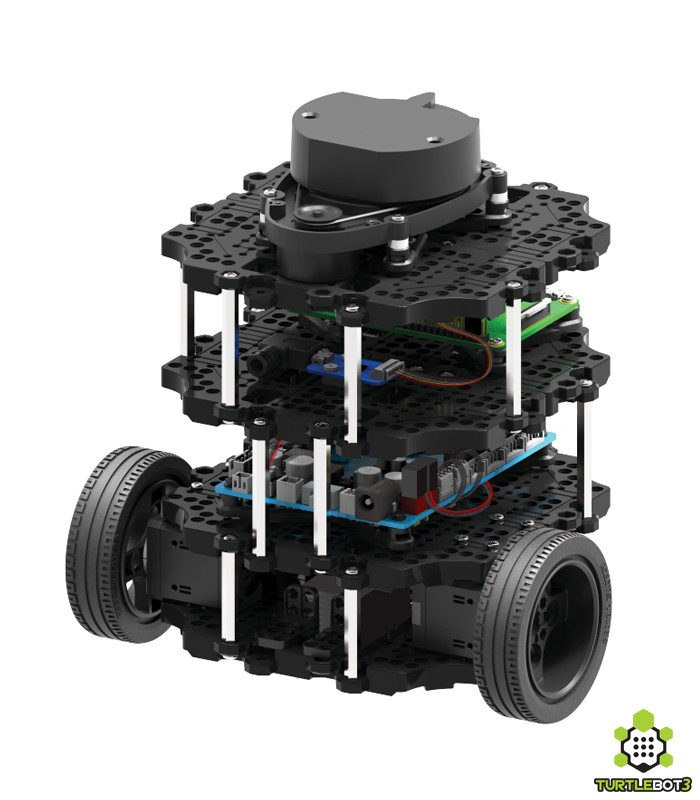
\includegraphics[width=0.8\textwidth]{Figures/ConAnalysis/General/Turtlebot3_burger.jpg}
\caption{The TurtleBot 3 Burger model}
\label{fig:TB3}
\end{figure}

%http://emanual.robotis.com/docs/en/platform/turtlebot3/appendix_lds_01/?fbclid=IwAR39-SkIJldceIYH9VY_rTEctMl9EI4fgVkyCGjcuvkLHvKBxIQptJJDy_0#user-guide-for-embedded-board


\section{Raspberry Pi 3}
Raspberry Pi 3 is a small single-board computer. It is capable of doing everything that a computer usually is able to do. It also has the ability to interact with the outside world, for example connecting with the cameras.\\

\begin{figure}[H]
\centering
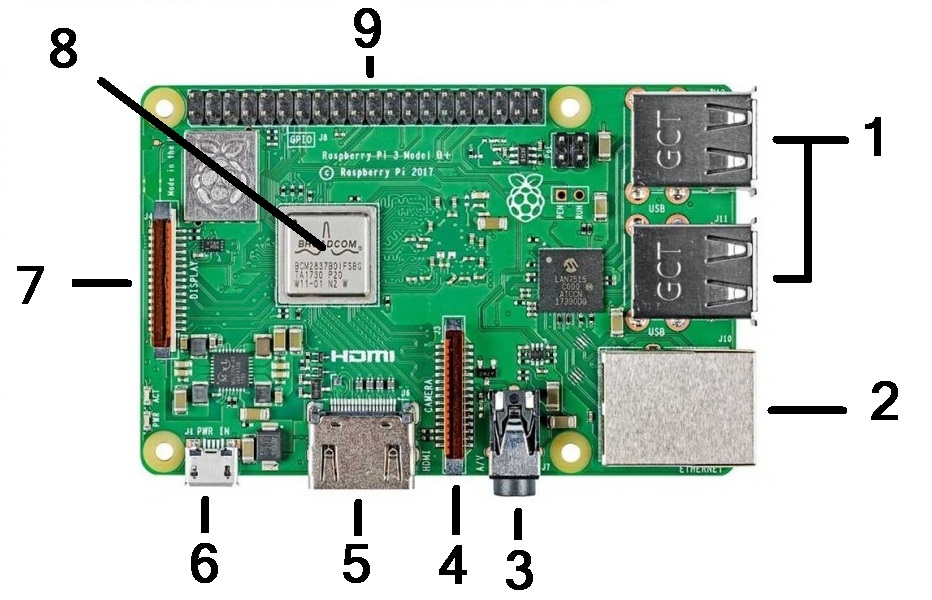
\includegraphics[width=0.8\textwidth]{Figures/ConAnalysis/General/RASBERRY.jpg}
\caption{Raspberry Pi 3 with components marked for reference beneath}
\label{fig:rasber}
\end{figure}

Raspberry Pi 3 model B, consist of four USB 2.0 ports (numbered as 1 in figure \ref{fig:rasber}). It has a LAN port (2) for network connection, it has a 3.5mm 4-pole composite video and audio output mini-jack (3). Furthermore, it has a CSI camera port (4) which finds the interface between camera and processor, a full-size HDMI video output (5) used for connection with a monitor and it has a micro USB input (6) used for powering the Raspberry Pi with up to 2.5 Amps. Moreover, the DSI display port (7) is used as a connector to a liquid crystal display panel. The main board for raspberry pi 3 is Broadcom BCM2837 (8) which has a 64bit processor, quad-core CPU at the 1.2GHz frequency and 1GB RAM (random access memory). Also, it has 40 pins extended GPIO (general-purpose input/output) (9) see picture \ref{fig:rasber}. Lastly, it has Bluetooth and Wi-Fi connection and Micro SD card slot underneath used as system memory.  \\

%https://docs-emea.rs-online.com/webdocs/162c/0900766b8162cdf1.pdf

%http://linuxgizmos.com/raspberry-pi-3-has-a-64-bit-cpu-but-a-32-bit-raspbian-os/

\section{Lidar} 
The Turtlebot 3 series come with the 2D, 360 degree laser scanner (Lidar), model LDS-01. The Lidar uses a laser diode projecting light with a bandwidth of 785nm to detect the surrounding 360 degrees of the sensor, in a 2D plain with the same elevation as the sensor. The laser used is of \textbf{"class 1"} and is as such safe \textit{"under all conditions of normal use"}\cite{Lasercla21:online}, but can pose a hazard in some extreme circumstances eg. if viewed through magnifying optics such as a microscope with a large aperture.\cite{2DLidar}
\begin{item}
\item It uses 3.3V USART, enabling it to transmit 230400 bytes per second (bps) and is full duplex. 
\item It functions in environments where the ambient light doesn't exceed 10.000 lux. For comparison full daylight (whiteout direct sun) is between 10.000 and 25.000 lux. 
\item It has a sampling rate of 1.8kHz.
\item It has a functional detection distance of between 12 cm and 3.5 m
\end{item}

\begin{figure}[H]
\centering
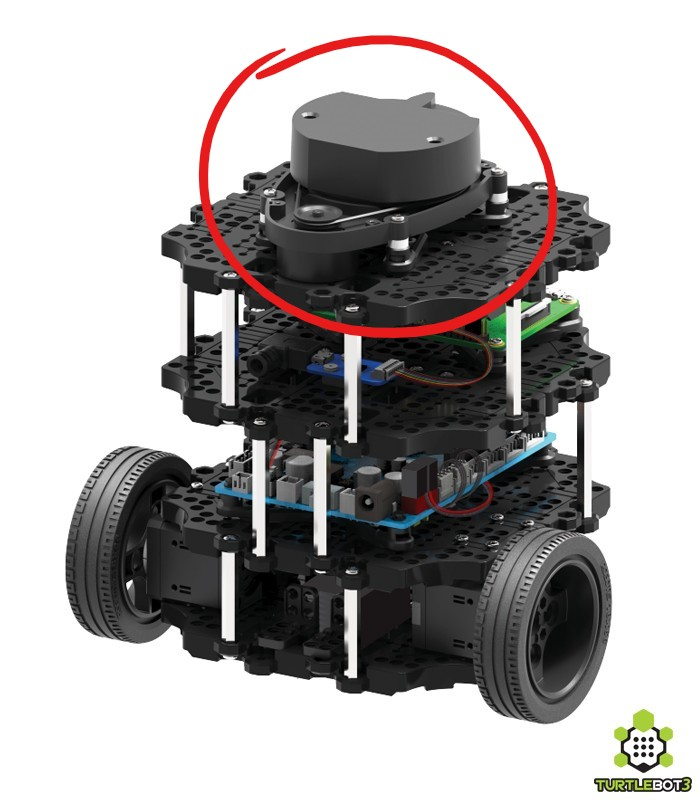
\includegraphics[width=0.8\textwidth]{Figures/ConAnalysis/General/Turtlebot3_burger-Lidar.jpg}
\caption{The TurtleBot 3 Burger model, with the Lidar encircled in red.}
\label{fig:TB3}
\end{figure}
\todo[inline]{fix a figure}


\section{Intel RealSense depth camera  D435}

RealSense depth camera D435 is USB-powered camera that includes a wider field of view depth sensors and an RGB sensor. The camera is used for capturing fast motion and the global shutter allows it to do so. Global shutter is a method which is used for moving objects and rapid movements sequences, where it "freezes" the moving object in place. The RealSense camera is used both in indoor and outdoor environment.\\ 

\begin{figure}[H]
\centering
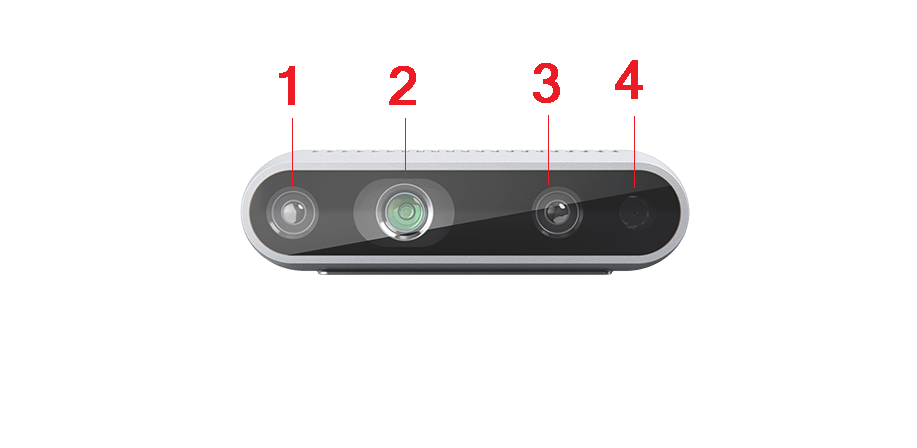
\includegraphics[width=0.8\textwidth]{Figures/ConAnalysis/General/real.png}
\caption{RealSence deep camera d435:\\ 1 and 3- Depth sensor \\ 2-Wide Infrared projector  \\ 4-RGB colour camera}
\label{fig:realsence}
\end{figure}

The camera has a range of 10 meters which depends on calibration, scene and lighting conditions. RGB is up to 1920*1080 resolution and has a frame rate of 30fps. Furthermore, the physical features of camera dimensions are length 90 mm, depth 25mm and height 25mm. Also a USB 3 is used for connection. \\

%https://realsense.intel.com/wp-content/uploads/sites/63/Intel_RealSense_D400_Family_Datasheet_Jan2019.pdf

\section{Dynamixel Motors} 
For the TurtleBot3, Dynamixel servos are used for the wheels. The model is XL430-W250. The control algorithm which the servo is using is a PID controller with a baud rate of 9600. It is possible to operate the servo in four different modes: Velocity, Position, Extended Position, and PWM. The servo uses Half-duplex Asynchronous Serial Communication as the Protocol Type, this means there can only be one way of communication at a time.\cite{DynamixelServo}
\color{black}